%!TEX root=../main.tex
\section{Results}
\label{sec:largeexact_results}

We compare the performance of exact Gaussian processes against widely-used scalable GP approximation methods on a range of large-scale datasets from the UCI dataset repository \cite{asuncion2007uci}.
Our experiments demonstrate that exact GPs:
\begin{enumerate*}
  \item outperform popular approximate GPs methods on nearly all benchmarking datasets in our study;
  \item compute thousands of test-point predictions in less than a second, even when $N > 10^6$;
  \item utilize all available data when making predictions, even when $N > 10^5$; and
  \item achieve linear training speedups on large datasets by adding additional GPU devices.
\end{enumerate*}

\paragraph{Baselines.}
We compare against two scalable GP approximations: Sparse Gaussian Process Regression (SGPR) \cite{titsias2009variational}, and Stochastic Variational Gaussian Processes (SVGP) \cite{hensman2013gaussian}.
We choose these methods due to their popularity and general applicability, enabling a comparison over a wide range of datasets.
We use $M = 512$ for SGPR and $M = 1,\!024$ for SVGP, which are common values used for these methods \cite{matthews2017gpflow}.
We later experiment with varying the number of inducing points.

\paragraph{Experiment details.}
Each dataset is randomly split into $75\%$ training, $10\%$ validating, and $15\%$ testing sets.
The data is whitened to be mean $0$ and standard deviation $1$ as measured by the training set.
We use a constant prior mean and a Mat\'ern 5/2 kernel with independent lengthscales for each dimension.

We train the learnable parameters of exact GPs and SGPR with $100$ iterations of Adam with a learning rate of $0.1$.
For SVGP, we perform $100$ epochs of Adam with a minibatch size of $1,\!024$ and a learning rate of $0.01$, which we find to perform better than $0.1$.
All exact and SGPR models use a rank-$100$ partial pivoted-Cholesky preconditioner and run PCG with a tolerance of $\Vert \trainK \bc - \by \Vert_2 / \Vert \by \Vert_2 = 1$ during training.
We constrain the learned noise to be at least $0.1$ to regularize the poorly conditioned kernel matrix for the houseelectric and Buzz datasets.

All training/evaluation experiments use a single NVIDIA GTX 2080-TI GPU unless otherwise stated.
We use the KeOps library \cite{charlier2020kernel} in conjunction with our GPyTorch BBMM/LOVE implementations to perform the partitioned kernel MVMs.
%We perform all training on one machine with 8 NVIDIA Tesla V100-SXM2-32GB-LS GPUs.

\begin{table}[!tb]
  \caption[Performance comparison between exact GPs and scalable approximations on large UCI datasets.]{
    Performance comparison between exact GPs and scalable approximations on large UCI datasets using ARD Mat\'ern kernels.
    All trials on $N < 100,\!000$ datasets are averaged over 3 trials; $\pm$ corresponds to 1 standard deviation.
    (We are unable to scale SGPR to HouseElectric due to its memory requirements when $m=512$.)
    {\bf Top:} test set root mean square error (RMSE).
    {\bf Bottom:} test set negative log likelihood (NLL).
  }
  \label{tab:large_exact_gp_results}
  \centering
  \vspace{1em}

  \resizebox{\textwidth}{!}{%
    \begin{tabular}{ cccccc }
  \toprule
  &&&
	\multicolumn{3}{c}{{\bf RMSE}}  \\
  \cmidrule{4-6}
  \thead{\\{\bf Dataset}} & \thead{\\$N$} & \thead{\\$D$} &
  \thead{{\bf Exact GP} \\ (BBMM)} & \thead{{\bf SGPR} \\ ($M\!=\!512$)} & \thead{{\bf SVGP} \\ ($M\!=\!1,\!024$)}
  \\
  \midrule
	PoleTele             & $9,\!600$          & $26$  &   $\mathbf{0.151}\pm 0.012$  & $0.217\pm 0.002$          & $0.215\pm 0.002$  \\
	Elevators            & $10,\!623$         & $18$  &   $\mathbf{0.394}\pm 0.006$  & $0.437\pm 0.018$          & $0.399\pm 0.009$  \\
	Bike                 & $11,\!122$         & $17$  &   $\mathbf{0.220}\pm 0.002$  & $0.362\pm 0.004$          & $0.303\pm 0.004$  \\
	Kin40K               & $25,\!600$         & $8$   &   $\mathbf{0.099}\pm 0.001$  & $0.273\pm 0.025$          & $0.268\pm 0.022$  \\
	Protein              & $29,\!267$         & $9$   &   $\mathbf{0.536}\pm 0.012$  & $0.656\pm 0.010$          & $0.668\pm 0.005$  \\
	KeggDirected         & $31,\!248$         & $20$  &   $\mathbf{0.086}\pm 0.005$  & $0.104\pm 0.003$          & $0.096\pm 0.001$  \\
	CTslice              & $34,\!240$         & $385$ &   $0.262\pm 0.448$           & $\mathbf{0.218}\pm 0.011$ & $1.003\pm 0.005$  \\
	KEGGU                & $40,\!708$         & $27$  &   $\mathbf{0.118}\pm 0.000$  & $0.130\pm 0.001$          & $0.124\pm 0.002$  \\
	3DRoad               & $278,\!319$        & $3$   &   $\mathbf{0.101}\pm 0.007$  & $0.661\pm 0.010$          & $0.481\pm 0.002$  \\
	Song                 & $329,\!820$        & $90$  &   $0.807\pm 0.024$           & $\mathbf{0.803}\pm 0.002$ & $0.998\pm 0.000$  \\
  Buzz                 & $373,\!280$        & $77$  &   $\mathbf{0.288}\pm 0.018$  & $0.300\pm 0.004$          & $0.304\pm 0.012$  \\
	HouseElectric        & $1,\!311,\!539$    & $9$   &   $\mathbf{0.055}\pm 0.000$  & -----                     & $0.084\pm 0.005$  \\
  \bottomrule
\end{tabular}

  }
  \vspace{1em}

  \resizebox{\textwidth}{!}{%
    \begin{tabular}{ cccccc }
  \toprule
  &&&
	\multicolumn{3}{c}{{\bf NLL}}  \\
  \cmidrule{4-6}
  \thead{\\{\bf Dataset}} & \thead{\\$N$} & \thead{\\$D$} &
  \thead{{\bf Exact GP} \\ (BBMM)} & \thead{{\bf SGPR} \\ ($M\!=\!512$)} & \thead{{\bf SVGP} \\ ($M\!=\!1,\!024$)}
  \\
  \midrule
	PoleTele             & $9,\!600$          & $26$  &    $-0.660\pm 0.081$          &  $-0.817\pm 0.005$             &  $\mathbf{-0.644}\pm 0.008$    \\
	Elevators            & $10,\!623$         & $18$  &     $0.626\pm 0.043$          &   $0.528\pm 0.015$             &   $\mathbf{0.486}\pm 0.019$    \\
	Bike                 & $11,\!122$         & $17$  &    $\mathbf{-1.323}\pm 0.170$ &  $-0.805\pm 0.005$             &  $-0.984\pm 0.021$             \\
	Kin40K               & $25,\!600$         & $8$   &    $\mathbf{-0.755}\pm 0.009$ &  $-0.073\pm 0.055$             &   $0.091\pm 0.033$             \\
	Protein              & $29,\!267$         & $9$   &     $0.960\pm 0.033$          &   $\mathbf{0.915}\pm 0.004$    &   $0.952\pm 0.018$             \\
	KeggDirected         & $31,\!248$         & $20$  &    $-0.838\pm 0.031$          &  $\mathbf{-1.163}\pm 0.005$    &  $-0.853\pm 0.033$             \\
	CTslice              & $34,\!240$         & $385$ &     $0.939\pm 0.004$          &  $\mathbf{-0.037}\pm 0.060$    &   $1.423\pm 0.005$             \\
	KEGGU                & $40,\!708$         & $27$  &    $-0.540\pm 0.035$          &  $\mathbf{-1.049}\pm 0.010$    &  $-0.653\pm 0.013$             \\
	3DRoad               & $278,\!319$        & $3$   &     $1.239\pm 0.025$          &   $0.791\pm 0.033$             &   $\mathbf{0.486}\pm 0.010$    \\
	Song                 & $329,\!820$        & $90$  &     $\mathbf{1.162}\pm 0.002$ &   $1.243\pm 0.083$             &   $1.417\pm 0.000$             \\
	Buzz                 & $373,\!280$        & $77$  &     $0.161\pm 0.026$          &   $\mathbf{0.092}\pm 0.017$    &   $0.119\pm 0.042$             \\
	HouseElectric        & $1,\!311,\!539$    & $9$   &    $\mathbf{-0.207}\pm 0.001$ & -----                          &   $0.024\pm 0.984$             \\
  \bottomrule
\end{tabular}

  }
  \vspace{1em}
\end{table}

\paragraph{Accuracy.}
\cref{tab:large_exact_gp_results} displays the accuracy and negative log likelihoods of exact GPs and approximate methods on several large-scale datasets.
We find that exact GPs achieve lower error than approximate methods on nearly every dataset.
Notably, on certain datasets like 3droad, exact GPs achieve a half or even a quarter of the error of some approximate methods.
Although \citet{nguyen2019exact} show results for exact GPs on $N \leq 120,\!000$, this is the first set of results comparing exact GPs to approximate GPs on $N\gg 10^5$.

Moreover, we also see that performance of the scalable GP methods is dataset dependent.
Neither SVGP nor SGPR consistently outperforms the other.
Interestingly, dataset size/dimensionality do not seem to influence the relative performance of approximate methods.
For example, though Protein and Kin40K are similar in size and have similar dimensionality, the approximate methods perform worse on Kin40K (relative to the RMSE of exact GPs).

\begin{table*}[t!]
  \vspace{1em}
  \caption[Wall-clock time comparison between exact GPs and approximate GPs on large UCI datasets.]{
    Wall-clock time comparison between exact GPs and approximate GPs on large UCI datasets.
    Models are trained and evaluated on a single NVIDIA GTX 2080-TI GPU.
    All trials on $N < 100,\!000$ datasets are averaged over 3 trials; $\pm$ corresponds to 1 standard deviation.
    {\bf Top:} training time for exact GPs and scalable approximations.
    {\bf Bottom:} prediction time for exact GPs.
    Precomputation refers to computing the LOVE cache.
    Prediction refers to computing the predictive distributions for $1,\!000$ test points.
  }
  \label{tab:large_exact_gp_timings}
  \centering
  \vspace{1em}

  \resizebox{\textwidth}{!}{%
    %!TEX root=../main.tex
\begin{tabular}{ cccccc }
  \toprule
  &&& \multicolumn{3}{c}{{\bf Training}}\\
  \cline{4-6}
  \thead{\\{\bf Dataset}} & $N$ & $D$ &
  \thead{{\bf Exact GP} \\ (BBMM)} &
  \thead{{\bf SGPR} \\ ($M\!=\!512$)} &
  \thead{{\bf SVGP} \\ ($M\!=\!1,\!024$)}
  \\
  \midrule
  PoleTele             & $9,\!600$          & $26$  &      $\mathbf{41.5}$ {\bf s}   $\mathbf{\pm}$ $\mathbf{1.1}$  &               $69.5$ s         $\pm$ $20.5$                     &       $68.7$ s   $\pm$ $4.1$    \\
	Elevators            & $10,\!623$         & $18$  &      $\mathbf{41.0}$ {\bf s}   $\mathbf{\pm}$ $\mathbf{0.7}$  &               $69.7$ s         $\pm$ $22.5$                     &       $76.5$ s   $\pm$ $5.5$    \\
	Bike                 & $11,\!122$         & $17$  &      $\mathbf{41.2}$ {\bf s}   $\mathbf{\pm}$ $\mathbf{0.9}$  &               $70.0$ s         $\pm$ $22.9$                     &       $77.1$ s   $\pm$ $5.6$    \\
	Kin40K               & $25,\!600$         & $8$   &      $\mathbf{42.7}$ {\bf s}   $\mathbf{\pm}$ $\mathbf{2.7}$  &               $97.3$ s         $\pm$ $57.9$                     &      $195.4$ s   $\pm$ $14.0$   \\
	Protein              & $29,\!267$         & $9$   &      $\mathbf{47.9}$ {\bf s}   $\mathbf{\pm}$ $\mathbf{10 }$  &              $136.5$ s         $\pm$ $53.8$                     &      $198.3$ s   $\pm$ $15.9$   \\
	KeggDirected         & $31,\!248$         & $20$  &      $\mathbf{51.0}$ {\bf s}   $\mathbf{\pm}$ $\mathbf{6.3}$  &              $132.0$ s         $\pm$ $65.6$                     &      $228.2$ s   $\pm$ $22.9$   \\
  CTslice              & $34,\!240$         & $385$ &               $3.32$ min       $\pm$ $5.0$                    &      $\mathbf{2.16}$ {\bf min} $\mathbf{\pm}$ $\mathbf{0.99}$   &       $3.86$ min $\pm$ $0.34$   \\
  KEGGU                & $40,\!708$         & $27$  &     $\mathbf{0.790}$ {\bf min} $\mathbf{\pm}$ $\mathbf{0.14}$ &               $2.22$ min       $\pm$ $1.0$                      &       $4.78$ min $\pm$ $0.40$   \\
  3dRoad               & $278,\!319$        & $3$   &               $15.8$ min       $\pm$ $7.4$                    &      $\mathbf{12.0}$ {\bf min} $\mathbf{\pm}$ $\mathbf{5.5}$    &       $34.0$ min $\pm$ $3.1$    \\
  Song                 & $329,\!820$        & $90$  &      $\mathbf{4.22}$ {\bf min} $\mathbf{\pm}$ $\mathbf{3.7}$  &               $7.88$ min       $\pm$ $3.1$                      &       $39.6$ min $\pm$ $3.1$    \\
  Buzz                 & $373,\!280$        & $77$  &               $1.19$ hr        $\pm$ $0.39$                   &      $\mathbf{0.486}$ {\bf hr} $\mathbf{\pm}$ $\mathbf{0.30}$   &      $0.772$ hr  $\pm$ $0.05$   \\
  HouseElectric        & $1,\!311,\!539$    & $9$   &      $\mathbf{1.20}$ {\bf hr}  $\mathbf{\pm}$ $\mathbf{0.04}$ &                -----                                            &      $6.12$  hr  $\pm$ $0.08$   \\
  \bottomrule
\end{tabular}

  }
  \vspace{1em}

  \resizebox{\textwidth}{!}{%
    \begin{tabular}{ cccccccc }
  \toprule
  &&& \multicolumn{1}{r}{\small\bf Precomputation} &&
  \multicolumn{3}{c}{{\bf Prediction}} \\
  \cline{4-4} \cline{6-8}
  \thead{\\{\bf Dataset}} & $N$ & $D$ &
  \thead{{\bf Exact GP} \\ (BBMM)} &&
  \thead{{\bf Exact GP} \\ (BBMM)} &
  \thead{{\bf SGPR} \\ ($M\!=\!512$)} &
  \thead{{\bf SVGP} \\ ($M\!=\!1,\!024$)}
  \\
  \midrule
	PoleTele             & $9,\!600$          & $26$  &  $5.14$ s    && $\mathbf{6}$ \textbf{ms}    & $\mathbf{6}$ \bf ms    & $273$ ms \\
	Elevators            & $10,\!623$         & $18$  &  $0.95$ s    && $\mathbf{7}$ \textbf{ms}    & $\mathbf{7}$ \bf ms    & $212$ ms \\
	Bike                 & $11,\!122$         & $17$  &  $0.38$ s    && $\mathbf{7}$ \textbf{ms}    & ${9}$ ms               & $182$ ms \\
	Kin40K               & $25,\!600$         & $8$   &  $12.3$ s     && $\mathbf{11}$ \textbf{ms}   & $       {12}$ ms       & $220$ ms \\
	Protein              & $29,\!267$         & $9$   &  $7.53$ s     && $       {14}$ ms            & $\mathbf{9}$ \bf ms    & $146$ ms \\
	KeggDirected         & $31,\!248$         & $20$  &  $8.06$ s    && $\mathbf{15}$ \textbf{ms}   & $       {16}$ ms       & $143$ ms \\
	CTslice              & $34,\!240$         & $385$ &  $7.57$ s   && $\mathbf{22}$ \textbf{ms}   & $       {14}$ ms       & $133$ ms \\
	KEGGU                & $40,\!708$         & $27$  &  $18.9$ s    && $\mathbf{18}$ \textbf{ms}   & $       {13}$ ms       & $211$ ms \\
	3dRoad               & $278,\!319$        & $3$   &  $118$ m*     && ${119}$ ms                  & $\mathbf{68}$ \bf ms   & $130$ ms \\
	Song                 & $329,\!820$        & $90$  &  $22.2$ m*   && ${123}$ ms                  & $\mathbf{99}$ \bf ms   & $134$ ms \\
	Buzz                 & $373,\!280$        & $77$  &  $42.6$ m*   && ${131}$ ms                  & $\mathbf{114}$ \bf ms  & $142$ ms \\
	HouseElectric        & $1,\!311,\!539$    & $9$   &  $3.40$ hr*   && ${958}$ ms                  & -----                  & $\mathbf{166}$ \textbf{ms} \\
  \bottomrule
\end{tabular}

  }

  \vspace{2em}
\end{table*}


\paragraph{Training time.}
\cref{tab:large_exact_gp_timings} displays the training time for exact and approximate GPs.
Datasets with $N \leq 100,\!000$ data points, exact GPs can be trained in minutes.
Datasets with $N \geq 100,\!000$ can be trained in hours.
While approximate GPs tend to be faster, we do note that the training time of exact GPs is within an order of magnitude of their approximate counterparts.
It is quite remarkable that exact GPs, which require $\bigo{N^2}$ computation with BBMM, are not much slower than $\bigo{N}$ approximate methods.
We hypothesize that exact GPs benefit more from GPU acceleration, as exact kernel matrices afford more MVM parallelism than approximate kernel matrices.

\paragraph{Prediction time.}
Although exact GPs take longer to train, we find that their speed is comparable to approximate methods at test time.
\cref{tab:large_exact_gp_timings} displays the time to compute $1,\!000$ predictive means and variances at test time before and after LOVE precomputation.
All predictions are made on one NVIDIA RTX 2080 Ti GPU.
We see exact GPs take \emph{milliseconds} across all dataset sizes used.

\begin{figure}[t!]
  \centering
  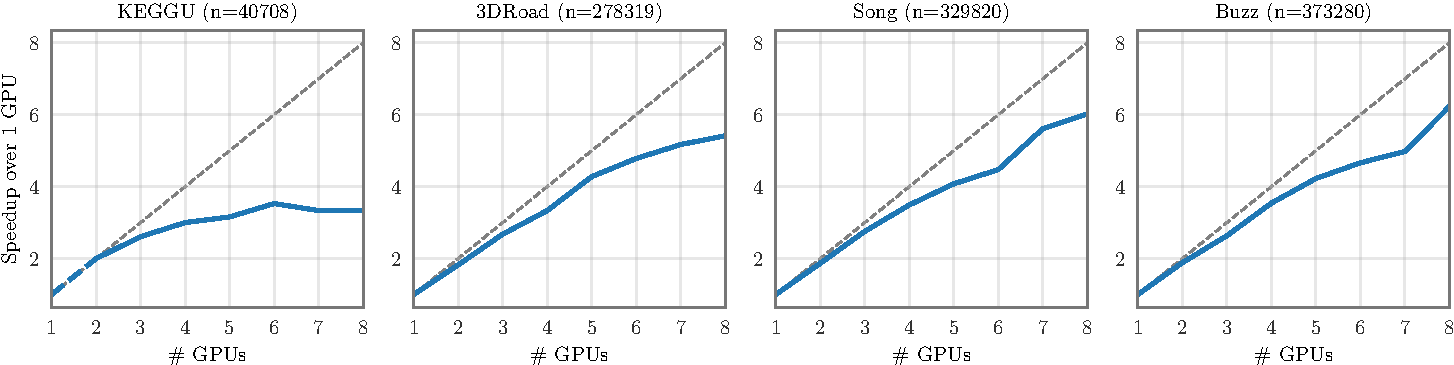
\includegraphics[width=0.70\linewidth]{figures/gpu_speedup.pdf}
  \caption[Speed of BBMM training using multi-GPU computation.]{
    Speed of BBMM training using multi-GPU computation.
    On large datasets, exact GPs with BBMM achieve a near linear speedup with more GPUs.
    (Speedups are measured on NVIDIA Tesla V100-SXM2-32GB-LS GPUs using models with non-ARD Mat\'ern 3/2 kernels.)
  }
  \label{fig:gpu_speedup}
\end{figure}

\paragraph{Training acceleration with multiple GPUs.}
As discussed in \cref{sec:largeexact_method}, the MVMs in BBMM and LOVE can be distributed across multiple devices.
\cref{fig:gpu_speedup} plots the speedup as more GPUs are used for training on the KEGGU, 3DRoad, Song, and Buzz datasets.
(Speedups are measured on NVIDIA Tesla V100-SXM2-32GB-LS GPUs using models with non-ARD Mat\'ern 3/2 kernels.)
Each of these datasets achieve a nearly linear speedup when adding up to 4 GPUs.
The speedup is more pronounced for the two large datasets (3DRoad and Song).


\subsection{Ablation Studies}
With BBMM and LOVE, we can better understand how exact GPs scale to datasets with $N\gg 10^4$ compared to approximate GPs.
Here, we demonstrate how the amount of data affects exact GP performance, and how the number of inducing points affects the performance of approximate GPs.
All experimental results in this section use GPs with non-ARD Mat\'ern 3/2 kernels.

\begin{figure}[t!]
  \centering
  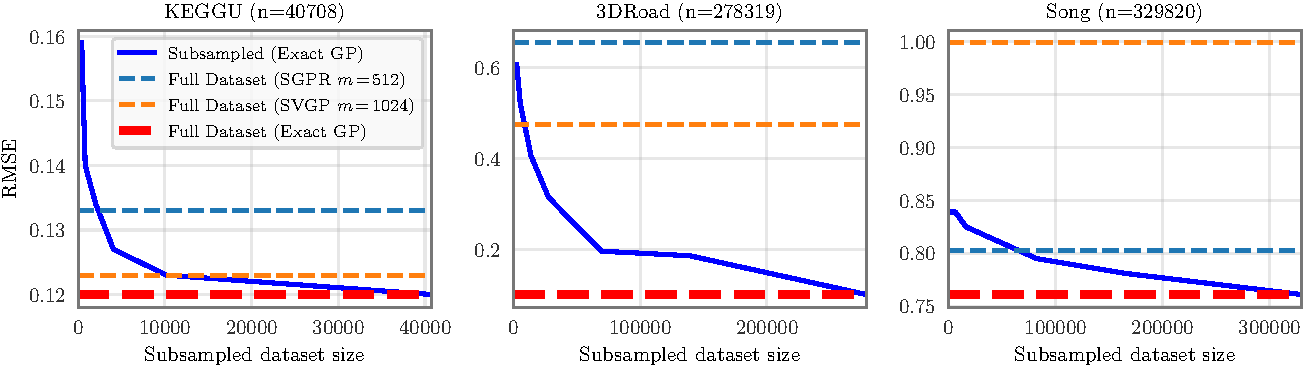
\includegraphics[width=0.7\linewidth]{figures/subsampling.pdf}
  \caption{
    Test root-mean-square error (RMSE) as a function of subsampled dataset size (lower is better).
    Subsampled exact GPs outperform approximate GPs even with a quarter of the training set.
    Exact GP error continues to decrease as data is added until the full dataset is used.
  }
  \label{fig:subsampling_results}
\end{figure}

\paragraph{Do GPs need the entire dataset?}
As a non-parametric model, Gaussian processes naturally adapt to the amount of training data available.
\cref{fig:subsampling_results} shows an increase in accuracy as we increase the amount of training data on the KEGGU, 3DRoad, and Song datasets.
For each dataset, we subsample a fraction of the training data and plot the resulting test set RMSE as a function of training set size.
As expected, the error decreases monotonically as we increase the subsample size.
\cref{fig:subsampling_results} also shows the performance of exact GPs, SGPR, and SVGP trained on the entire dataset.
Strikingly, in all three cases, \textit{an exact GP with less than a quarter of the training data outperforms approximate GPs trained on the entire training set}.
Test error continues to decrease with the addition of training data.

\begin{figure}[!t]
  \centering
  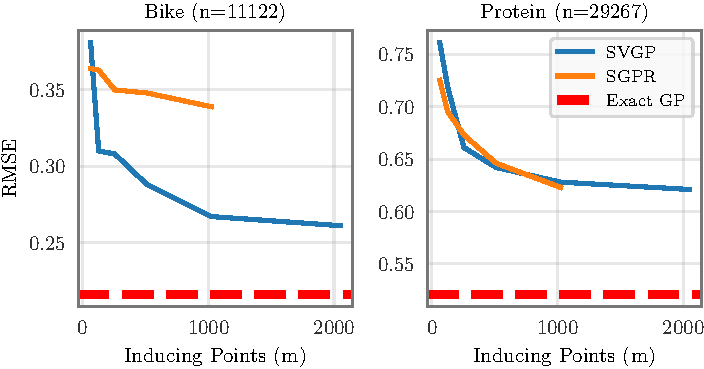
\includegraphics[width=0.7\linewidth]{figures/inducing_points.pdf}
  \caption{
    Error of SVGP and SGPR methods as a function of the number of inducing points
    ($m$).  Both methods scale cubically with $m$.
    We were unable to run SGPR with more than $1,\!024$ inducing points on a single GPU.
    Exact GPs have lower error than both methods.
  }
  \label{fig:num_inducing_points}
\end{figure}

\paragraph{Would more inducing points help?}
The results in \cref{tab:large_exact_gp_results} naturally raise the question: ``can approximate models with more inducing points recover the performance of exact methods?''
In \cref{fig:num_inducing_points}, we plot test set RMSE on two datasets, Bike and Protein, as a function of the number of inducing points.
The test RMSE of SGPR and SVGP saturates on both datasets well above the test RMSE of an exact GP.
We note that using $M$ inducing points introduces a $M \times M$ matrix and a $\bigo{NM^2 + M^3}$ time complexity \cite{hensman2013gaussian,hensman2015scalable} which makes it difficult to train SGPR with $M \gg 1024$ inducing points.
It is possible to combine partitioned kernel MVMs with inducing-point methods to utilize even larger values of $M$.
However, as \cref{fig:num_inducing_points} and \cref{tab:large_exact_gp_results} show, it may be preferable to use the extra computational resources to train an exact GP on more data rather than to train an approximate GP with more inducing points.
